% !TEX TS-program = XeLaTeX
% use the following command:
% all document files must be coded in UTF-8
\documentclass[portuguese]{textolivre}
% build HTML with: make4ht -e build.lua -c textolivre.cfg -x -u article "fn-in,svg,pic-align"

%\usepackage{hyperref}

\journalname{Texto Livre}
\thevolume{17}
%\thenumber{1} % old template
\theyear{2024}
\receiveddate{\DTMdisplaydate{2023}{1}{24}{-1}} % YYYY MM DD
\accepteddate{\DTMdisplaydate{2023}{4}{10}{-1}}
\publisheddate{\DTMdisplaydate{2023}{11}{2}{-1}}
\corrauthor{Frederico Araújo Durão}


\articledoi{10.35699/1983-3652.2024.42708}
%\articleid{NNNN} % if the article ID is not the last 5 numbers of its DOI, provide it using \articleid{} commmand 
% list of available sesscions in the journal: articles, dossier, reports, essays, reviews, interviews, editorial
\articlesessionname{articles}
\runningauthor{Santos et~al.} 

\sectioneditorname{Leonardo Carneiro Araujo}
\layouteditorname{Frederico Araújo Durão}

\title{Um sistema de recomendação baseado em conteúdo para adoção de animais utilizando a técnica do cosseno ponderado}
\othertitle{A content-based recommendation system for animal adoption using the weighted cosine technique}
% if there is a third language title, add here:
%\othertitle{Artikelvorlage zur Einreichung beim Texto Livre Journal}

\author[1]{Monaliza Carvalho Santos\orcid{0000-0001-7117-812X}\thanks{Email: \href{mailto:monaliza.carvalho@ufba.br}{monaliza.carvalho@ufba.br}}}

\author[1]{Lorena Lima da Silveira dos Santos\orcid{0009-0005-8295-3976}\thanks{Email: \href{mailto:lorena.lima@ufba.br}{lorena.lima@ufba.br}}}

\author[1]{Vítor Hugo Barbosa dos Santos\orcid{0000-0002-1771-2624}\thanks{Email: \href{mailto:vitorbarbosa@ufba.br}{vitorbarbosa@ufba.br}}}

\author[1]{Guilherme Souza Brandão\orcid{0000-0002-7217-0231}\thanks{Email:\href{mailto:guilhermebrandao@ufba.br}{guilhermebrandao@ufba.br}}}

\author[1]{Frederico Araújo Durão\orcid{0000-0002-7766-6666}\thanks{Email: \href{mailto:fdurao@ufba.br}{fdurao@ufba.br}}}

\affil[1]{Universidade Federal da Bahia, Salvador, BA, Brasil.}

\addbibresource{article.bib}
% use biber instead of bibtex
% $ biber article


% used to create dummy text for the template file
\definecolor{dark-gray}{gray}{0.35} % color used to display dummy texts
\usepackage{lipsum}
%\setlipsum{\colorlet{oldcolor}{.}\color{dark-gray}}{\color{oldcolor}}
\setlipsum{%
  par-before = \begingroup\color{dark-gray},
  par-after = \endgroup
}
\usepackage{algorithm}



\usepackage{algpseudocode}

% used here only to provide the XeLaTeX and BibTeX logos
\usepackage{hologo}

% if you use multirows in a table, include the multirow package
\usepackage{multirow}

% provides sidewaysfigure environment
\usepackage{rotating}

% CUSTOM EPIGRAPH - BEGIN 
%%% https://tex.stackexchange.com/questions/193178/specific-epigraph-style
\usepackage{epigraph}
\renewcommand\textflush{flushright}
\makeatletter
\newlength\epitextskip
\pretocmd{\@epitext}{\em}{}{}
\apptocmd{\@epitext}{\em}{}{}
\patchcmd{\epigraph}{\@epitext{#1}\\}{\@epitext{#1}\\[\epitextskip]}{}{}
\makeatother
\setlength\epigraphrule{0pt}
\setlength\epitextskip{0.5ex}
\setlength\epigraphwidth{.7\textwidth}
% CUSTOM EPIGRAPH - END
% LANGUAGE - BEGIN
% ARABIC
% for languages that use special fonts, you must provide the typeface that will be used
% \setotherlanguage{arabic}
% \newfontfamily\arabicfont[Script=Arabic]{Amiri}
% \newfontfamily\arabicfontsf[Script=Arabic]{Amiri}
% \newfontfamily\arabicfonttt[Script=Arabic]{Amiri}
%
% in the article, to add arabic text use: \textlang{arabic}{ ... }
%
% RUSSIAN
% for russian text we also need to define fonts with support for Cyrillic script
% \usepackage{fontspec}
% \setotherlanguage{russian}
% \newfontfamily\cyrillicfont{Times New Roman}
% \newfontfamily\cyrillicfontsf{Times New Roman}[Script=Cyrillic]
% \newfontfamily\cyrillicfonttt{Times New Roman}[Script=Cyrillic]
%
% in the text use \begin{russian} ... \end{russian}
% LANGUAGE - END

% EMOJIS - BEGIN
% to use emoticons in your manuscript
% https://stackoverflow.com/questions/190145/how-to-insert-emoticons-in-latex/57076064
% using font Symbola, which has full support
% the font may be downloaded at:
% https://dn-works.com/ufas/
% add to preamble:
% \newfontfamily\Symbola{Symbola}
% in the text use:
% {\Symbola }
% EMOJIS - END

% LABEL REFERENCE TO DESCRIPTIVE LIST - BEGIN
% reference itens in a descriptive list using their labels instead of numbers
% insert the code below in the preambule:
%\makeatletter
%\let\orgdescriptionlabel\descriptionlabel
%\renewcommand*{\descriptionlabel}[1]{%
%  \let\orglabel\label
%  \let\label\@gobble
%  \phantomsection
%  \edef\@currentlabel{#1\unskip}%
%  \let\label\orglabel
%  \orgdescriptionlabel{#1}%
%}
%\makeatother
%
% in your document, use as illustraded here:
%\begin{description}
%  \item[first\label{itm1}] this is only an example;
%  % ...  add more items
%\end{description}
% LABEL REFERENCE TO DESCRIPTIVE LIST - END


% add line numbers for submission
%\usepackage{lineno}
%\linenumbers
\begin{document}
\maketitle


\begin{polyabstract}
\begin{abstract}
A adoção animal é considerada um gesto grandioso que carrega consigo grande responsabilidade social, visto que um animal precisa dos cuidados e carinho diário do adotante. Muito além da aparência e questões estéticas, é essencial que o adotante considere suas reais condições respeitando as características específicas do animal. A falta de perícia na escolha do animal pode acarretar uma adoção irresponsável e infrutuosa, comprometendo a qualidade de vida do animal. Portais de adoção de animais são suscetíveis a esse problema se não fornecerem mecanismos que tentem aproximar as reais preferências e condições do adotante com as características do animal. Diante dessa problemática, este artigo propõe um sistema de recomendação baseado em conteúdo que visa sugerir animais para adoção considerando as preferências dos adotantes, aplicando a técnica do cosseno ponderado. A ponderação é fundamental no cálculo de similaridade entre as preferências dos adotantes e das características do animal. Os experimentos realizados apontam um aumento de precisão das recomendações quando a ponderação é aplicada sobre o método tradicional sem considerar as preferências do adotante por determinadas características dos animais a serem adotados. 

\keywords{Sistema de recomendação \sep Recomendação baseada em conteúdo \sep Adoção de animais \sep Adoção de cães \sep Técnica do cosseno ponderado}
\end{abstract}

\begin{english}
\begin{abstract}
An adopted animal is considered a grand gesture with significant social responsibility since it needs daily care and affection from the adopter. Far beyond appearance and aesthetic issues, the adopter must consider their natural conditions, respecting the specific characteristics of the animal. The lack of expertise in choosing the animal can lead to an irresponsible and fruitless adoption, compromising the animal's quality of life. Animal adoption portals are prone to this problem if they do not provide controls that try to approximate the adopter's real motivations and conditions with the animal's characteristics. Faced with this problem, this article proposes a content-based recommendation system to suggest animals for users to consume drugs, applying the weighted cosine technique. The weighting is fundamental in calculating the similarity between the users' emotions and the animal's characteristics. The experiments increased the accuracy of the recommendations when weighting is applied over the traditional method without considering the prescribed method of users by specific characteristics of the animals to be adopted.

\keywords{Recommender system \sep Content-based recommendation \sep Adoption of animals \sep Dog adoption \sep Weighted cosine technique}
\end{abstract}
\end{english}
% If there is another abstract, insert it here using the same scheme
\end{polyabstract}

\section{Introdução}\label{sec-intro}
Uma pesquisa feita pelo Instituto Brasileiro de Opinião Pública e Estatística \textcite{IBOPE} revelou que o brasileiro abandona seus animais de estimação por motivos fúteis e os compra sem pensar nas implicações. Baseado nos dados do estudo, o professor da Faculdade de Medicina Veterinária da Universidade de São Paulo (USP), Ricardo Dias, fez um alerta: \textit {"Os sinais são preocupantes. Mostram que o brasileiro procura animal de estimação baseado em modismos de raça e tem baixa propensão a tentar manter o animal, diante de mudanças no estilo de vida”.} De acordo com a mesma pesquisa, 42\% dos adotantes de cães e gatos, no Brasil, não castram seus \textit{pets} \cite{RECMVZ16221}. 

Nos Estados Unidos da América (EUA), as causas referidas para a devolução de cães em abrigos foram, primeiramente, problemas comportamentais dos animais (46,8\% dos casos) e, em segundo lugar, mudanças na disponibilidade de espaço ou nas regras de conduta social do local ocupado pelo ser humano (29,1\%). Ainda como causas importantes de abandono, constam o estilo de vida do adotante (25,4\%) e as expectativas criadas por ele — sejam elas emocionais, físicas ou sociais — a preparação desse novo adotante para a chegada do animal e a realidade nos cuidados do cão \cite{RECMVZ16221}.

Na América Latina, por exemplo, o abandono de animais é considerado uma forte ameaça nas áreas de saúde pública (devido às zoonoses), social (desconforto com relação ao comportamento animal), ecológica (principalmente no que se refere ao impacto ambiental) e econômica (custos com a estratégia de controle populacional). No que tange às questões de saúde, animais de rua são transmissores de doenças como raiva, leishmaniose, leptospirose, toxocariose, entre outras doenças parasitárias. Há também problemas como ruídos (latidos e uivos), excreções (fezes e urina) e acidentes de trânsito \cite{RECMVZ16221}.
Do mesmo modo, os impactos do abandono no bem-estar animal são igualmente relevantes. A situação mais frequente se caracteriza por condições de saúde física e mental deficientes, agravadas pela maior suscetibilidade a estados de sofrimento e exposição a maus tratos \cite{Stafford2007}.

Diante disso, a adoção pode ser promovida de várias formas, em feiras locais, aplicativos e sites de instituições governamentais, por exemplo. Porém, esses meios têm potencial de resultar numa busca árdua, tendo em vista a quantidade de animais disponíveis, ou numa má escolha, ocasionando adoções insatisfatórias e possíveis abandonos. Neste cenário, é perceptível a necessidade de aplicação de mecanismos inteligentes que filtrem conteúdos de forma personalizada, segundo as preferências de cada adotante.

Assim, conforme \textcite{Ricci2011}, é viável utilizar Sistemas de Recomendação - SR, empregando ferramentas de \textit{software} e técnicas que retornam sugestões de itens que provavelmente são de interesse do adotante. O termo "item", neste caso, é aplicado para referenciar o que o sistema recomenda ao adotante, como músicas, livros etc. Em face dessas observações, portanto, este trabalho propõe um SR que visa apresentar animais de acordo com as preferências do adotante, ponderando-as consoante o grau de importância. Essas preferências estão associadas ao estilo de vida do possível adotante, como o tipo de moradia (apartamento ou casa), a presença de crianças em casa e a disponibilidade para passear. Serviços inteligentes de apoio à adoção são oportunidades existentes devido às práticas tradicionais de recomendação — como pedir indicação de serviço ou produto para algum conhecido que já o consumiu —, uma vez que temos o hábito de atribuir confiança a quem nos indica algo, principalmente se esta vier de alguém próximo. Um serviço de recomendação, dessa forma, é um tipo de serviço inteligente, eficiente e confiável, pois sugere itens similares aos interesses de um determinado adotante.

Ao adotar um animal de estimação, geralmente, os futuros adotantes não sabem ou nem se informam sobre as características do bicho, buscando apenas algum que seja agradável esteticamente. Nesse contexto, o papel do SR é apresentar um item (animal) que mais se encaixe ao perfil do adotante, tendo em conta diversos aspectos, para que não se arrependa ou queira se desfazer futuramente. Sabe-se que há muitos animais disponíveis para adoção nos variados abrigos de uma cidade. O adotante, nesta situação, teria que fazer uma extensa pesquisa para achar o ideal e, ainda assim, correria o risco de não obter todas as informações necessárias para se fazer uma boa escolha. A busca poderia ser cansativa e trabalhosa e, no final, o “bicho aspirado”, resultante da pesquisa, pode já ter sido adotado durante o período das avaliações. Dessa maneira, assim como se utiliza as recomendações de produtos, também é possível recorrer à indicação de possíveis animais para adoção, conforme o perfil do adotante e do bicho. Este, então, terá um novo lar e um novo adotante, e o adotante terá um amigo condizente com o próprio estilo de vida.

A proposta descrita nesse trabalho é a de um SR para adoção de cães. A ideia é cadastrar cães disponíveis para adoção e permitir que os adotante  recebam sugestões de cães que correspondam com seu perfil, ou seja, que sejam compatíveis com suas preferências, necessidades e estilo de vida. O objetivo é aumentar as chances de sucesso na adoção, utilizando a técnica do cosseno ponderado, uma extensão da técnica de similaridade de cosseno, que consiste em atribuir um peso ou importância relativa aos atributos buscados pelo possível adotante. O diferencial desta proposta, para aquelas que já estão disponíveis, é a recomendação do cão ideal para determinado adotante considerando o grau de relevância das características. Não há literatura suficiente no Brasil e na América Latina que relacione fatores ao abandono de animais \cite{RECMVZ16221}. Em Taiwan, algumas das variáveis ligadas ao abandono estão associadas aos problemas comportamentais dos animais domésticos 
\cite{Weng:2006}. Ainda neste estudo, têm-se outras causas relativas ao insucesso na adoção, tais como a motivação da posse (aquisição do animal por estética) ou a falta de conhecimento sobre os animais.

O problema que este trabalho busca resolver, portanto, é a capacidade de recomendar um \textit{pet} baseada no grau de relevância de cada uma das características do adotante, aumentando, desta forma, a probabilidade de uma adoção bem sucedida, em vez da compra. E, embora a utilização do algoritmo de Similaridade do Cosseno proporcione a combinação de todas as qualidades do item e do adotante, não há garantias de melhor recomendação, posto que, daquela gama de combinações, algumas podem não ser relevantes para interferir na escolha mais assertiva de adoção do animal. 

Normalmente, os aplicativos \textit{mobile} e os \textit{sites} disponíveis para adoção de cães e gatos não fazem sugestões. Estas, contudo, são um fator importante, pois ajudam o futuro adotante a decidir acertadamente, sem intensas buscas, e evitam surpresas e frustrações posteriores — tais como um cão de grande porte para uma pessoa que mora em um pequeno apartamento, ou um cachorro manso e preguiçoso para ser um cão de guarda.

Este trabalho está organizado da seguinte maneira: A Seção \ref{cap:recsys} apresenta o referencial teórico sobre Sistemas de Recomendação e a Seção \ref{cap:tecadocao} traz os conceitos referentes às tecnologias de apoio à adoção de animais. Os trabalhos relacionados são discutidos na Seção \ref{cap:tr}. A Seção \ref{cap:tecadocao} detalha a arquitetura do sistema de recomendação bem como os algoritmos. A Seção \ref{cap:recsysadocao} apresenta a avaliação experimental, e a Seção \ref{cap:conclusion} conclui o trabalho e aponta os trabalhos futuros.

\section{Sistemas de recomendação}
\label{cap:recsys}

Quando o acesso à informação começou a ser facilitado através da \emph{Web}, o compartilhamento de dados passou a ser multiplicado. Os \textit{sites} de notícia, serviços de \emph{streaming} de música e vídeo, \emph{e-commerce} etc. utilizaram a indicação para filtrar o oferecimento de grande quantidade de informações de interesse do adotante. Os sistemas de recomendação funcionam, portanto, como salva-vidas nesse mar de dados. Sem eles, diante de tantas opções, fazer uma boa escolha poderia custar tempo, principalmente quando a pessoa possui pouca experiência de decisão em meio a inúmeras alternativas.

Para discutir sobre os sistemas de recomendação é preciso voltar no tempo, quando o primeiro SR era um tradicional sistema de filtragem e recuperação de informação, o Tapestry \cite{Goldberg:1992:UCF:138859.138867}, um sistema experimental de filtração de \emph{e-mails}, desenvolvido em 1992, por Xerox Palo Alto Research Center (PARC). O Tapestry era baseado em filtragem colaborativa, sendo o primeiro a usar o termo, e permite pesquisar \emph{e-mails} segundo o conteúdo do documento e as reações registradas de outros adotantes. E, diferente dos demais sistemas do período, o Tapestry não apenas examinava o \emph{e-mail} quando ele chegava, mas exibia anotações registradas por pessoas que já consultaram aquele \emph{e-mail}. No entanto, apesar de ser fundamentado em filtragem colaborativa, utilizava a de conteúdo \cite{Goldberg:1992:UCF:138859.138867}; isto é, no final, filtrava hibridamente. Assim, além da colaboração humana, lidava com palavras comuns contidas nos \emph{e-mails}.


Em sua publicação na revista da ACM, \textcite{Resnick:1997:RS:245108.245121} preferem utilizar o termo SR, uma vez que defendem que as recomendações podem sugerir itens preferencialmente relevantes e indicar quais devem ser filtrados sem necessitar da colaboração de pessoas. Desses itens recomendados, os adotantes podem fornecer \emph{feedbacks} implícito ou explícito, com um simples clique. Uma metodologia típica para fornecer esse \emph{feedback} é na forma de classificações, na qual os indivíduos selecionam valores numéricos de um sistema de avaliação específico — o sistema de classificação de cinco estrelas, por exemplo \textcite{Aggarwal2016} —, assim como foi utilizado neste estudo. Outras formas de retornos podem ser manipuladas de forma implícita, nas quais o adotante fornece dados para a recomendação de uma forma fácil, como o caso da \emph{Amazon} e outros comerciantes \emph{online}, com a compra ou navegação em itens \cite{Aggarwal2016}.


O Sistema de Recomendação é uma ferramenta de \textit{software} e técnicas que fornecem sugestões de itens para serem úteis ao adotante \cite{Ricci2011}. Um SR normalmente se concentra em um tipo específico de item (tais como filmes e músicas) e, consequentemente, o \textit{design} e a técnica de recomendação principal, utilizados para gerar as sugestões, são todos personalizados, a fim de fornecer indicações adequadas e eficazes para aquele item particular \cite{Ricci2011}. Os SRs referem-se, basicamente, a três tipos de objetos, apresentados abaixo:

\begin{itemize}
    \item \textbf{Itens:} os artigos que são recomendados. Podem ser caracterizados pela complexidade, valor ou utilidade. O valor de um item pode ser positivo, se é útil para o usuários, ou negativo, se não é apropriado ou foi escolhido erroneamente pelo próprio indivíduo. São apresentados a partir de várias abordagens de representação e informação; o filme, por exemplo, é o item a ser sugerido na \emph{Netflix}.

\item \textbf{Usuários:} têm uma variedade de objetivos e características. Os SRs extraem um conjunto de informações deles para personalizar as indicações. Essa seleção será modelada pelo sistema a depender da técnica de recomendação. 

\item \textbf{Transações:} são os registros de interações entre o usuário e o SR, usados pelos algoritmos de recomendação do sistema para encontrar e gerar sugestões úteis ao usuário — como navegar em um item e dar '\emph{like}' ou '\emph{deslike}'.
\end{itemize}
     
     
\subsection{Tarefas de um sistema de recomendação}

Após definir o que é um SR, serão detalhadas cada função que um SR pode desempenhar. Baseando-se no artigo de \textcite{Ricci2011}, que diferencia as tarefas de um SR dos provedores de serviços que fazem uso das recomendações, tem-se as seguintes atribuições: 

\begin{itemize}
    \item \textbf{Aumentar o número de itens vendidos:} considerada como a principal função de um SR comercial, deve ser capaz de vender um conjunto adicional de itens em comparação àqueles normalmente vendidos sem qualquer tipo de indicação. Esse objetivo é alcançado porque os itens recomendados, provavelmente, atendem as necessidades e desejos do usuário.
    
     \item \textbf{Vender itens mais diversificados:} selecionar e oferecer itens que podem ser difíceis de encontrar sem uma sugestão precisa.
     
     \item \textbf{Elevar a satisfação do usuário:} a combinação de recomendações acertadas e uma interface utilizável impulsionarão a avaliação e o aproveitamento do usuário no sistema.
     
     \item \textbf{Amplificar a fidelidade do usuário:} quanto mais tempo a pessoa interage com o sistema, mais refinado seu modelo de usuário se torna; ou seja, melhor será a  representação do sistema sobre suas preferências.
      
      \item \textbf{Entender melhor o desejo do usuário:} ter uma boa descrição dos interesses de quem usa o serviço, podendo ser reaproveitada em outros aplicativos. Um provedor de serviços pode, então, decidir utilizar esse conhecimento para outros objetivos.
     
\end{itemize}

 Em seguida, listam-se onze tarefas que um SR pode auxiliar a implementar para apoiar o usuário em suas escolhas, segundo \textcite{Herlocker:2004:ECF:963770.963772}, uma referência clássica:


\begin{itemize}
    \item \textbf{Encontrar alguns itens bons:} recomendar ao usuário alguns itens, como uma lista classificada, com alguma forma de avaliar o quanto gostou de determinado item — por exemplo, uma escala de cinco estrelas.
    
    \item \textbf{Encontrar todos os itens bons:} sugerir todos os itens que podem satisfazer as necessidades do usuário. Em alguns casos, é insuficiente localizar alguns itens bons quando a quantidade é relativamente pequena.
    
    \item \textbf{Anotação em contexto:} dada uma lista de itens, evidenciar alguns, de acordo com as preferências do usuário.
    
    \item \textbf{Recomendar uma sequência:} em vez de focar na geração de uma única recomendação, a ideia é indicar uma sequência de itens que seja agradável.
    
    \item \textbf{Recomendar um grupo:} recomendar um grupo de itens que combinem entre si.
    
    \item \textbf{Apenas navegar:} o sistema deve ajudar o usuário a navegar pelos itens, numa seção específica, com maior probabilidade de se enquadrar no escopo dos seus interesses.
    
    \item \textbf{Encontrar Sistema de Recomendação confiável:} para obter confiança do usuário, os sistemas também podem oferecer funções singulares, a fim de permitir que testem seu comportamento além daqueles essenciais para conseguir recomendações.
    
    \item \textbf{Melhorar o perfil:} o usuário pode fornecer informações, para o SR, sobre o que ele gosta ou não. Essa é uma tarefa fundamental para que o sistema seja capaz de fornecer sugestões personalizadas.
    
    \item \textbf{Expressar-se:} alguns usuários podem não se importar com as indicações. Nesse caso, o importante é que possam contribuir com suas avaliações e manifestar suas opiniões e crenças. Desse modo, o sistema deve ofertar um campo para comentários.
    
    \item \textbf{Ajudar os outros:} algumas pessoas ficam felizes em ajudar com informações, tal qual avaliar itens que eles tenham conhecimento ou experiência. Esse tipo de usuário acredita que a comunidade se beneficia de sua colaboração.
    
    \item \textbf{Ajudar os outros:} certos indivíduos têm como objetivo influenciar explicitamente outros a comprar determinados produtos. Também existem aqueles mal-intencionados que podem usar o sistema para promover ou penalizar itens.
    
\end{itemize}


\subsection{Desafios de um sistema de recomendação}

Os modelos básicos de sistemas de recomendação utilizam dois tipos de técnicas: (1) interações usuário-item, como avaliações ou comportamento de compra, e (2) as informações do perfil de usuários, como itens textuais ou palavras-chave relevantes \cite{Aggarwal2016}. O SR vai oferecer sugestões individualizadas como saída, ou será capaz de guiar o indivíduo de forma particularizada objetivando encontrar itens úteis \cite{Burke:2007}.

Nesta seção, serão explicados os dois principais tipos de sistemas de recomendação encontrados na literatura: as abordagens baseadas em filtragem colaborativa e a de conteúdo. Ressalta-se, contudo, a existência de outros tipos de técnicas como as de conhecimento, demográfica, social e a grupal \cite{Burke:2007}.

\subsubsection{Filtragem colaborativa}

Considerada a técnica mais popular e amplamente implementada nos SRs, a filtragem colaborativa recomenda ao usuário ativo os itens que outros indivíduos com gostos similares avaliaram positivamente \cite{Ricci2011}. O sistema localiza usuários pares com um histórico de classificação semelhante ao do usuário atual e gera recomendações utilizando esta vizinhança \cite{Burke:2007}.


Em \textcite{Burke:2007}, a filtragem colaborativa é dividida em dois métodos, baseados em vizinhança e modelo. O método de vizinhança se concentra nas relações entre os itens ou, alternativamente, entre usuários. Já o modelo molda a preferência de um usuário por um item a partir de elementos semelhantes avaliados pela mesma pessoa \cite{Ricci2011}. 


Um SR popular que utiliza filtragem colaborativa é a \emph{Netflix}. Ela ordena as recomendações de modo que os itens mais ranqueados estejam facilmente visíveis para os usuários, no topo da lista, na tentativa de serem selecionados pelo usuário Figura \ref{fig:001}. A mesma estratégia é usada para definir qual tipo de \emph{thumbnail} será apresentado ao usuário por meio de suas preferências \cite{Azevedo:2018}.

\begin{figure}[H]
	\centering
	\includegraphics[scale=1.10]{imagens/fig-025.png}
	\caption{Demonstração da lista de recomendação da Netflix. }
 \source{\cite{Azevedo:2018}}

	\label{fig:001}
\end{figure}

\subsubsection{Filtragem baseada em conteúdo}

Um SR embasado em conteúdo aprende a indicar itens semelhantes àqueles que o usuário avaliou bem. A correspondência dos itens é calculada segundo os atributos associados aos itens comparados \cite{Ricci2011}; além de calcular a equivalência entre os itens com características do usuário, que podem ser encontradas em um perfil. Esse tipo de SR analisa um conjunto de atributos dos itens previamente classificados pelo indivíduo ou, até mesmo, do perfil do usuário e, a partir disso, criam um modelo de interesses daquela pessoa \cite{Zhang2019}.


O padrão criado é uma representação das preferências do indivíduo, adaptado para encontrar e indicar novos itens que podem ser relevantes. O processo de sugestão consiste em comparar os atributos do modelo do usuário com os atributos de um item. Se um modelo reflete com precisão as preferências do usuário, isso é uma grande vantagem para a eficácia do processo de recomendação \cite{Lops:2011} (\Cref{fig:002}).

\begin{figure}[H]
	\centering
	\includegraphics[scale=0.60]{imagens/fig-026.png}
	\caption{Demonstração da recomendação baseada em conteúdo. }
 \source{\cite{daSilva:2019}}
	\label{fig:002}
\end{figure}


\subsubsection{Comparação das técnicas de recomendação}

Todas as técnicas de recomendação utilizadas na implementação de um SR possuem seus prós e contras. Seja nas informações do usuário, dos itens, na quantidade de dados, e avaliações, tudo pode influenciar o sucesso ou fracasso de uma técnica utilizada para implementação do algoritmo de sugestões do SR.

Conforme apresentado por \textcite{Burke:2007} e discutido por \textcite{Mladenic:1999}, seguem alguns pontos comuns das diferenças entre essas duas ferramentas:

\begin{itemize}
    \item \textbf{Baseada em conteúdo}: a principal vantagem desta é não precisar de \emph{feedback} prévio para começar a recomendar algo útil, pois, na falta de registros, o sistema monta um modelo de usuário com as informações de perfil, de cadastro ou de algum item avaliado no passado. A Figura \ref{fig:002} demonstra isso graficamente, o conteúdo B, similar ao A, será recomendado ao usuário.
    A desvantagem é que cria uma bolha de indicações, gerando uma lista muito similar, com pouca variedade. Outra desvantagem é que o sistema não vai gerar boas recomendações, se o usuário não possuir alguma característica que possa rotulá-lo, ou se não tiver avaliado anteriormente algum item no sistema.
    
    
    \item \textbf{Filtragem colaborativa}: não gera boas recomendações caso haja escassez de dados ou se os itens não tiverem apreciações de usuários diferentes. Porém, possui uma grande vantagem: a técnica resolve os principais problemas da recomendação baseada em conteúdo: não cria uma bolha de sugestões e não necessita de informações sobre o perfil ou um modelo de usuário, visto que não utiliza a similaridade entre itens para indicar.

\end{itemize}

\label{sec:conceitosSistemaRecomendacao}



\section{Tecnologia no apoio à adoção de animais} 
\label{cap:tecadocao}

Segundo \textcite{Gomes}, animais abandonados estão suscetíveis a riscos como maus tratos que, apesar de crime, não são punidos adequadamente. Além do sofrimento animal, o desamparo causa outros sérios problemas, como a proliferação de doenças transmissíveis para humanos, tais como a raiva e a leishmaniose. Animais em situação de abandono geram riscos à saúde pública, aumento dos gastos públicos, superlotação em Organizações Não Governamentais (ONG) e nos centros de zoonoses.

Para acolher esses bichos em vulnerabilidade, conforme citado por \textcite{Matos}, surgem as ONGs que desempenham um papel essencial na luta pela causa animal e, juntamente com protetores independentes, atuam resgatando, tratando e servindo de lar transitório. Porém, a quantidade de abandono é grande, e, assim, muitas instituições abrigam mais animais do que a infraestrutura permite. Por isso, devido à superlotação, muitos defensores acabam transformando a própria casa em abrigo temporário, o que pode não garantir uma boa assistência ao animal. 

Muitos dos recolhidos pelos centros de zoonoses brasileiros não são resgatados e adotados pela população. Dessa forma, acabam sendo submetidos à eutanásia, em virtude dos custos gerados ao cofres públicos pela manutenção em canis \cite{GARCIA-RODRIGUEZ2008} e pela falta de recursos para tratar as doenças e infecções que a maioria apresenta. Contudo, até mesmo a eutanásia exige despesas, conforme descrito na Resolução nº 174 do Conselho Federal de Medicina Veterinária (CFMV), com a compra de medicamentos, seringas e agulhas; além da contratação de médico-veterinário e da construção de um ambiente adequado para a realização do procedimento.

Por isso,  a utilização da tecnologia intenciona favorecer e apoiar o acesso dos interessados em ter um animal de estimação à adoção, desencorajando a compra. Entende-se que retirar um bicho da situação de abandono é um benefício não somente para o animal, mas para as ONGs que, geralmente, encontram-se lotadas — visto que a entrada de animais é, muitas vezes, maior que a saída —, para o ser humano, submetido às doenças transmitidas por animais de rua, e aos cofres públicos, que precisam realizar a eutanásia como forma mais rápida de “solucionar” o problema.

\subsection{Tecnologias no apoio à adoção}

Tecnologias, a nível de \textit{software} e/ou \textit{hardware}, já são utilizadas na identificação e controle para ajudar ONGs no resgate e na adoção de animais em situação de abandono, reduzindo o número de bichos tutelados por essas instituições. Algumas dessas tecnologias são empregadas para fins de controle, como os \textit{microchips} implantados em bois para manejo de rebanho.

Um trabalho realizado por \textcite{webmedia_estendido} buscou pesquisas que objetivavam diminuir o abandono e melhorar a divulgação de animais para adoção na região da Associação dos Municípios da Região da Foz do Rio Itajaí (AMFRI). Dentre as fases do estudo, encontra-se uma etapa em que foi feita uma pesquisa de campo e o desenvolvimento de um sistema \textit{web}. A investigação realizada levantou algumas tecnologias para apoiar o resgate de animais domésticos em situação de rua. Ainda segundo os autores \textcite{webmedia_estendido}, algumas inovações já são comumente utilizadas no suporte e na solução de problemas de reconhecimento e proteção do animal, evitando a perda deste. É o caso do \textit{microchip} \textit{Radio Frequency Identification (RFID)}, da Figura \ref{fig:003}, que consiste em um método de identificação através de sinais de rádio, cujos chips armazenam informações que podem ser lidas por leitores de etiquetas eletrônicas. O RFID é muito utilizado em controle de estoque, rastreamento de pacientes em hospitais e na contenção do rebanho, na agricultura.

\begin{figure}
	\centering
	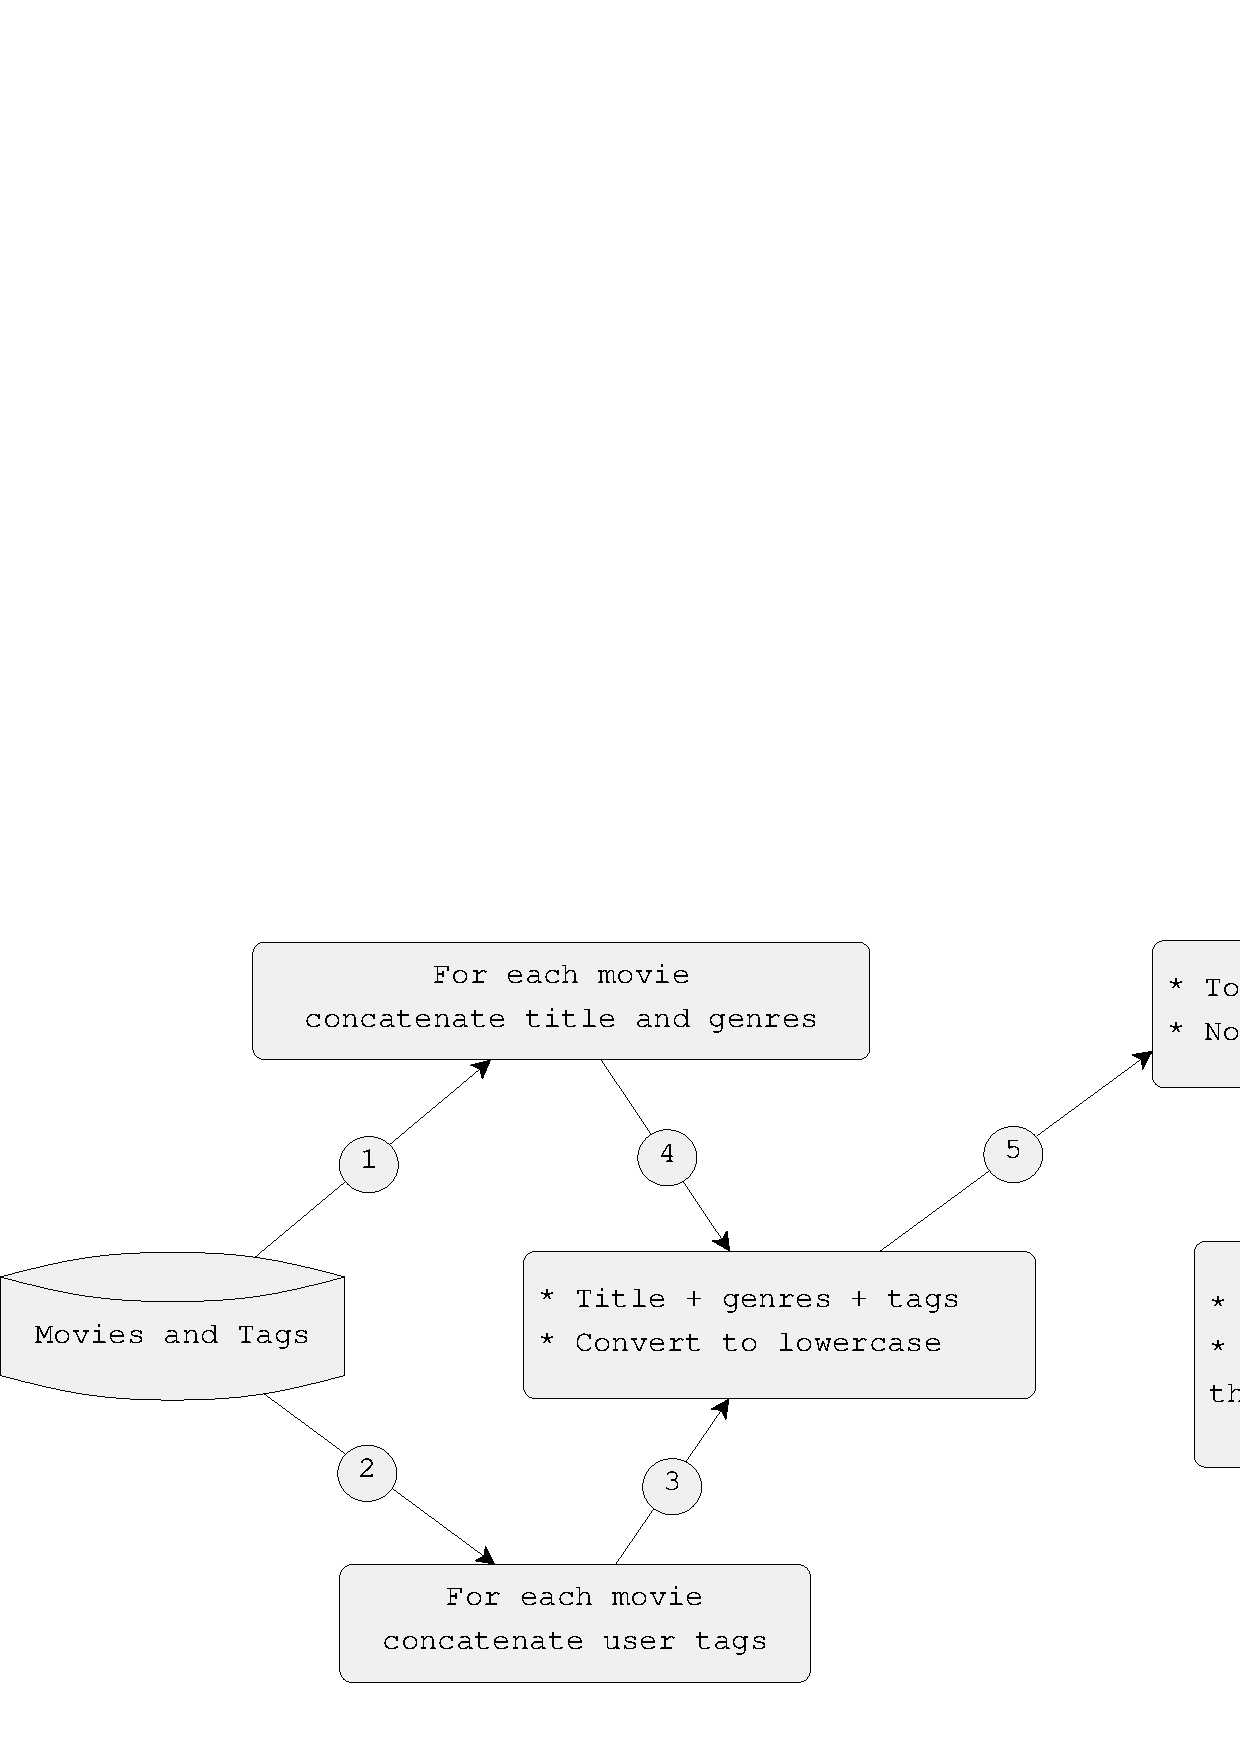
\includegraphics[scale=0.50]{imagens/fig-003.jpeg}
	\caption{Etiqueta RFID utilizada no Unleashed Indoor Dog Park.}
 \source{\cite{webmedia_estendido}.}
	\label{fig:003}
\end{figure} 

Outra tecnologia é a coleira com \textit{Quick Response Code - QR Code} Figura \ref{fig:004}, inserido no mercado pela \textit{FurCode}. Consiste numa coleira com medalha de identificação com \textit{QR Code}, que possibilita acessar a página do animal. Por meio desta, a pessoa que encontrar o animal utilizando a coleira pode ter acesso às informações de contato do adotante, telefone do médico veterinário, fotos e informações médicas. Além do \textit{QR Code}, a medalha pode conter o link da página do animal, para caso o indivíduo que o encontre não tenha acesso a um dispositivo que lê esse tipo de código.

A utilização de \textit{microchips} em animais também tem favorecido a adoção responsável. Consoante notícia publicada pelo \textcite{G1CE:2019}, em Fortaleza, a Coordenadoria Especial de Proteção e Bem-Estar Animal (Coepa), da Prefeitura de Fortaleza, está implantando \textit{microchips} em cães e gatos que foram adotados em eventos de adoção realizados na cidade. Até julho de 2019, 1.977 animais receberam o dispositivo e entraram para o banco de dados do órgão. O objetivo da iniciativa é acompanhar os animais adotados para evitar possíveis abandonos.

\begin{figure}
	\centering
	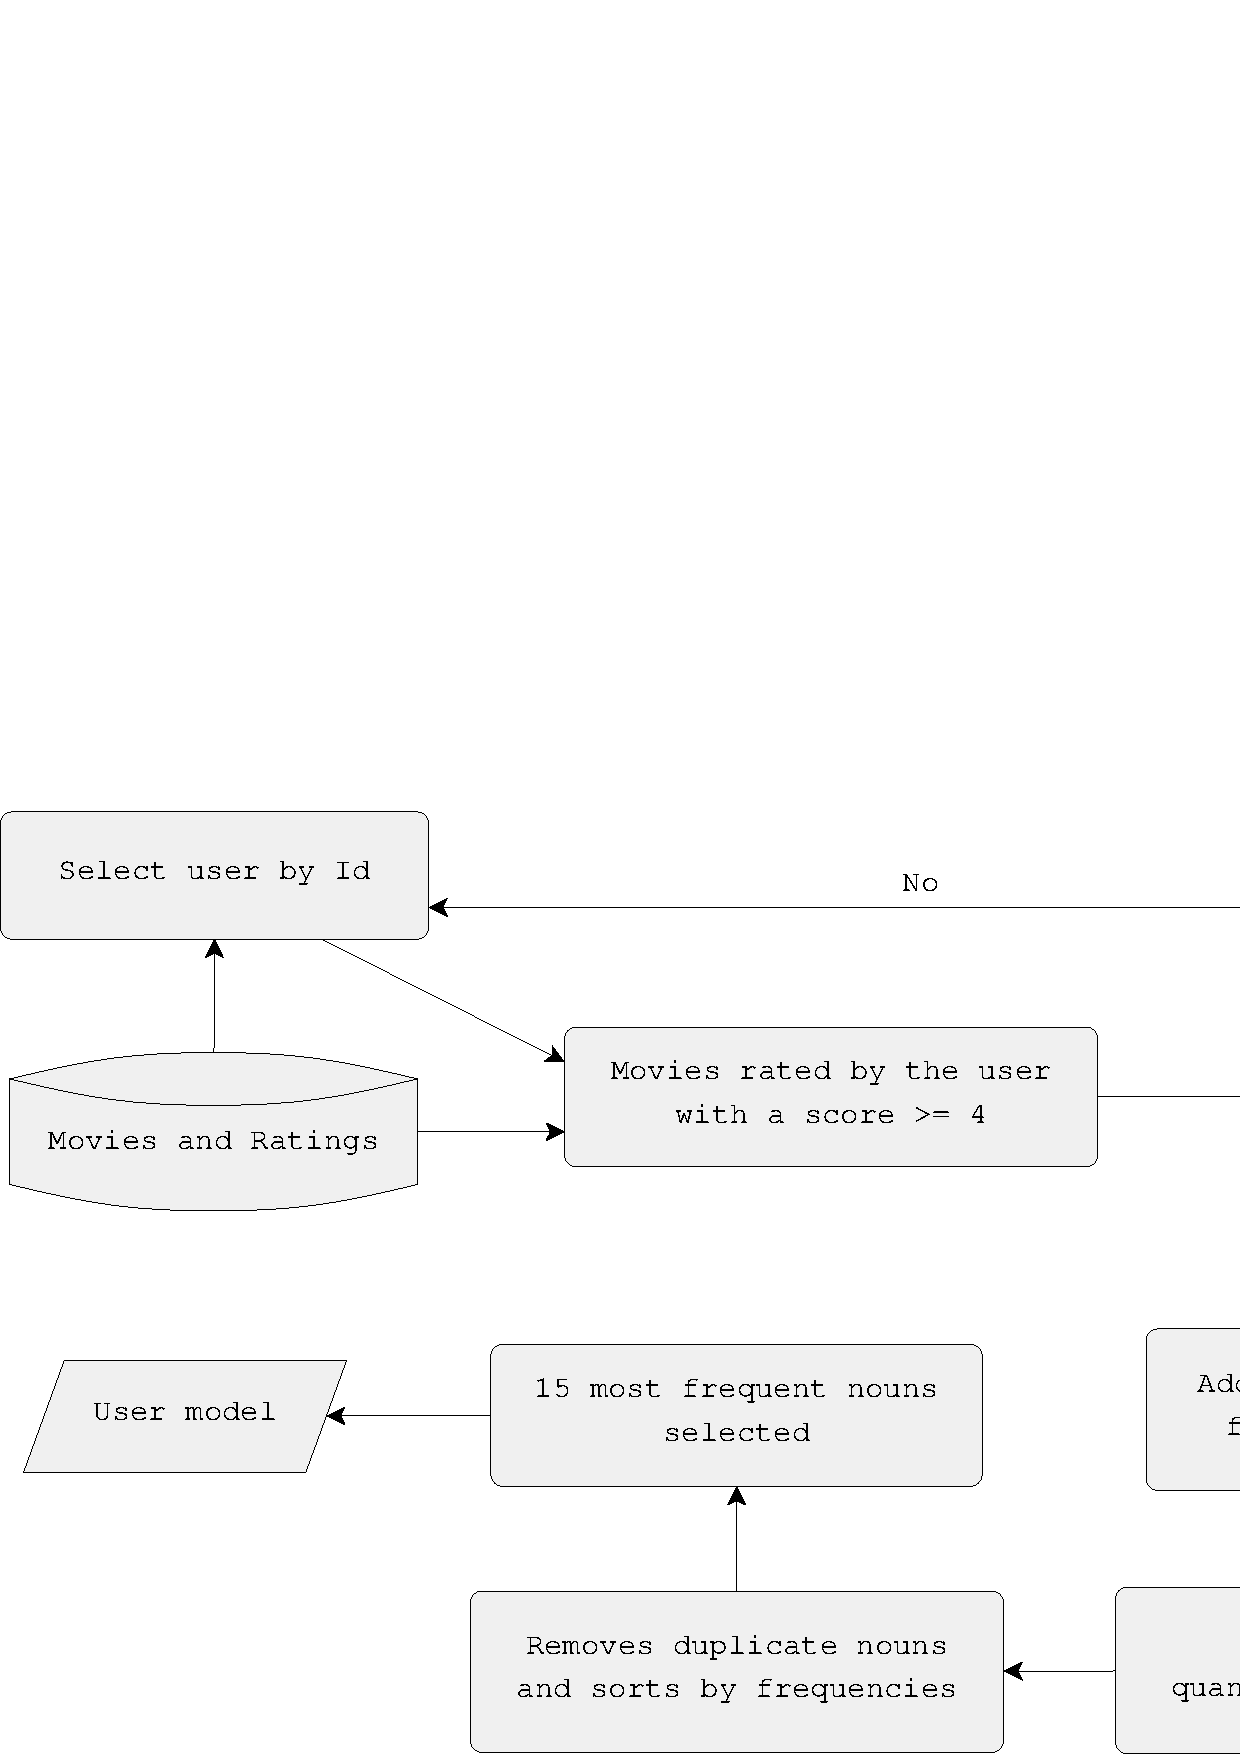
\includegraphics[scale=0.80]{imagens/fig-004.png}
	\caption{Coleira com \textit{QR Code} da FurCode.}
 \source{\cite{ColeiraQRCODE}.}
	\label{fig:004}
\end{figure} 

\subsection{Sistemas e iniciativas de apoio à adoção de \textit{pets}}

Os aplicativos de busca também são utilizados para cadastrar animais que tenham fugido de casa ou se perderam de seus adotantes. Através deste cadastro, os adotantes inserem fotos e informações do animal desaparecido e os dados de contato. Há o exemplo do \textit{app} \textit{Petfinder Adoptable Pets}, visto na Figura \ref{fig:005} e disponível para \textit{Android} e \textit{iOS}, que se constitui num \textit{app} de busca de  perdidos e abandonados. A interface conta um mapa mostrando os animais disponíveis mais próximos do adotante.

\begin{figure}
	\centering
	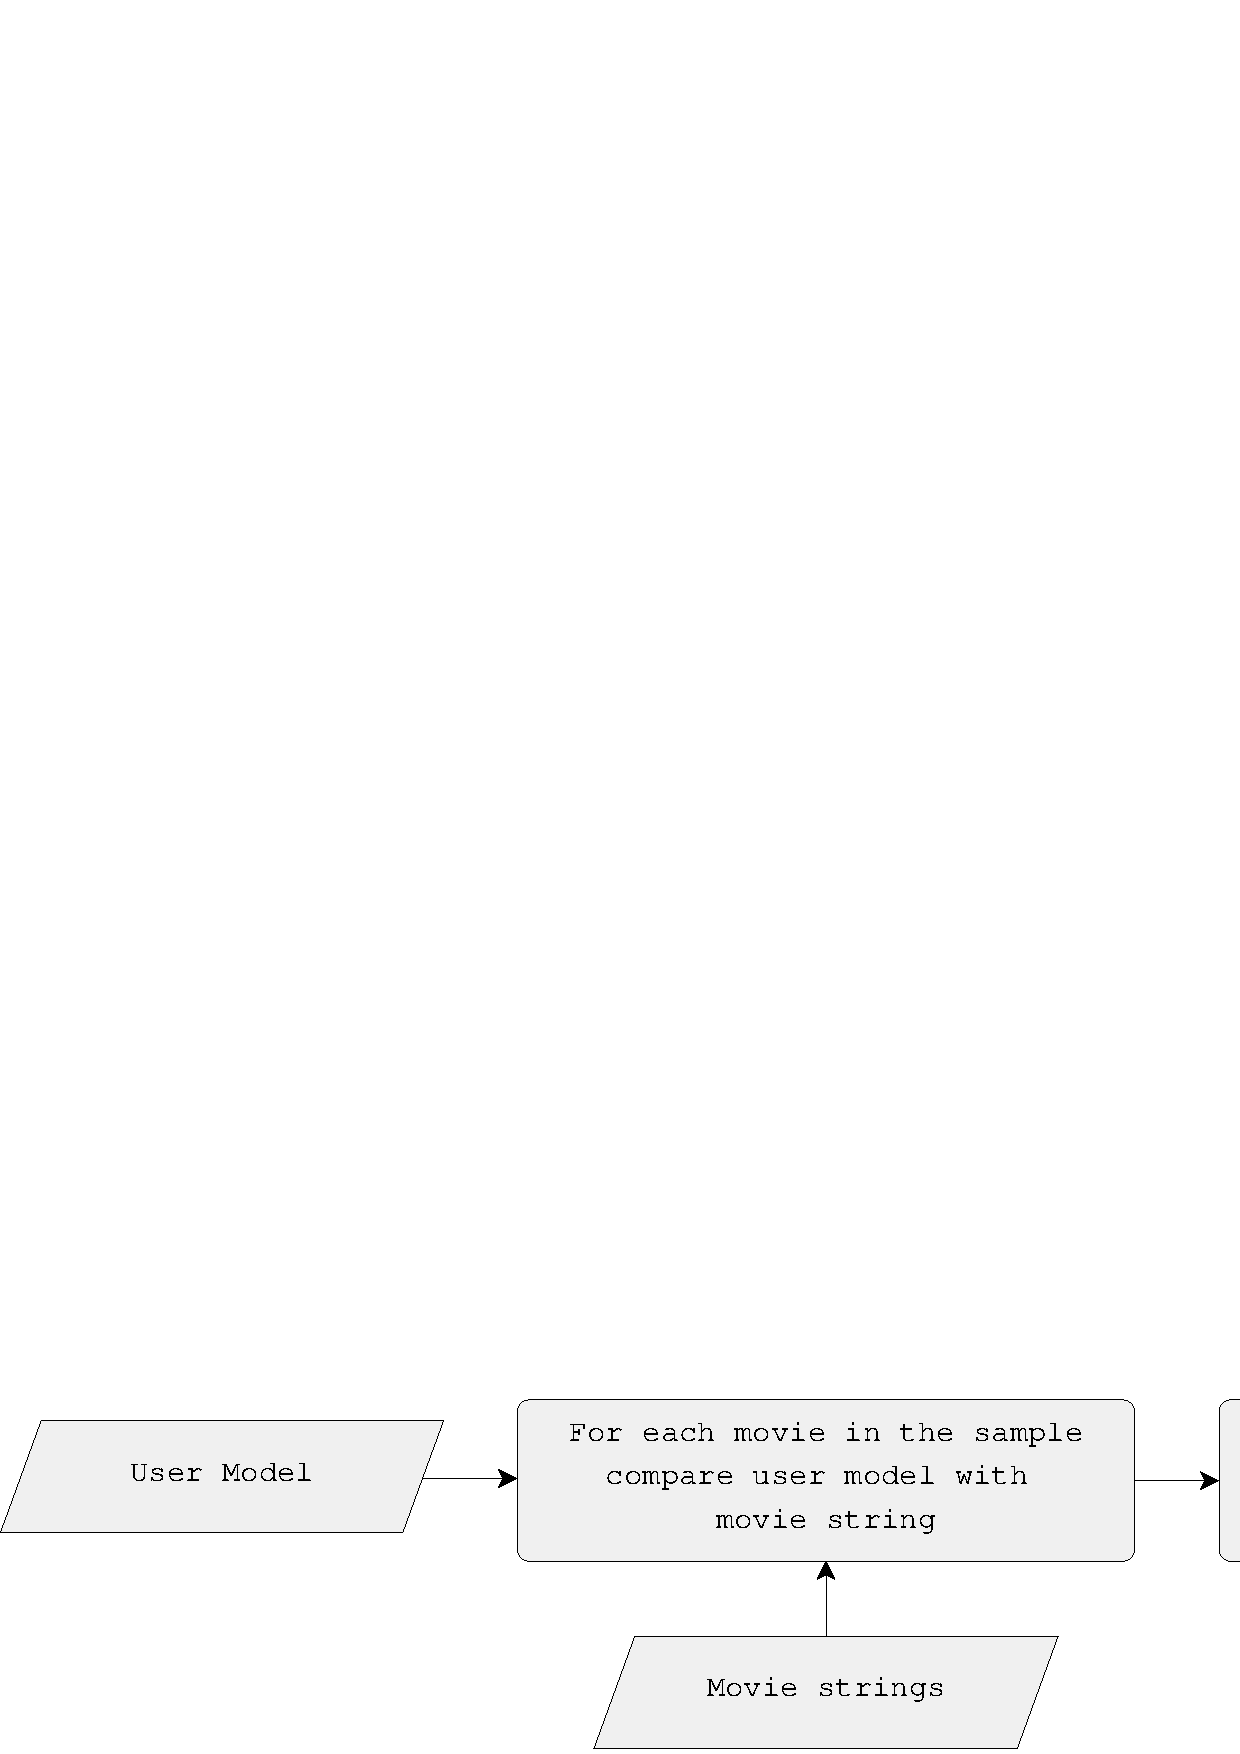
\includegraphics[scale=0.80]{imagens/fig-005.png}
	\caption{Tela de busca do app \textit{Petfinder Adoptable Pets}}
 \source{\textcite{petfinderdogsforadotion}}
	\label{fig:005}
\end{figure} 

Outra alternativa são os aplicativos de identificação de animal que a promovem por meio de recognição facial, utilizando a tecnologia de comparação de imagens (visão computacional e inteligência artificial), como é o caso do app \textit{Crowdpet}\footnote{App desenvolvido pela \textit{SciPet}, uma das empresas-filhas da Universidade Estadual de Campinas (Unicamp).}, apresentado na Figura \ref{fig:007}.  Segundo notícia publicada pela \textcite{FAPESP:2017}, o aplicativo cruza duas fontes de dados: as fotos dos animais perdidos cadastradas por seus adotantes e as fotos de animais avistados nas ruas por voluntários. Usa, assim, reconhecimento facial para buscar combinações entre as características de cães e gatos achados e perdidos.

Uma aplicação que também usa identificação facial foi desenvolvida pela \textit{startup} chinesa \textit{Megvii}, Figura \ref{fig:006}, que fornece soluções para recognição da face ao programa de vigilância do governo da China. Conforme publicação de \textcite{Tecmundo:2022}, o \textit{app} identifica rostos de animais de estimação através de impressões lidas no nariz de cães, espécies de impressões digitais, para gerar um banco de dados que ajuda a localizar animais perdidos.

\begin{figure}
	\centering
	\includegraphics[scale=0.70]{imagens/fig-006.png}
	\caption{Telas do \textit{app} chinês de reconhecimento facial.}
 \source{\cite{TheVerge}.}
	\label{fig:006}
\end{figure}

\begin{figure}
	\centering
	\includegraphics[scale=0.70]{imagens/fig-007.png}
	\caption{App \textit{Crowdpet} cruza características de fotos publicadas de animais achados e perdidos.}
 \source{\cite{Today}.}
	\label{fig:007}
\end{figure}

Quando se pensa em adotar um \textit{pet}, atualmente, basta pesquisar na \textit{Web} alguma instituição governamental ou portal da prefeitura municipal que disponibiliza animais para adoção. Essas informações já se encontram facilmente disponíveis, trazendo, algumas vezes, a descrição das características físicas e comportamentais dos animais, assim como podem informar se o animal já é vermifugado, vacinado, castrado etc. Algumas instituições públicas e ONGs possuem seu próprio meio de disponibilizar dados sobre os animais a serem adotados, através de \textit{apps} \textit{mobile} ou \textit{web sites}. Isso torna mais prático promover a adoção naquela determinada região, sem que os indivíduos tenham que se deslocar para conhecer os animais e suas características relevantes.

Nos Estados Unidos a \textit{American Society for the Prevention of Cruelty to Animals} \cite{MYM:2017}, utiliza o \textit{Geographic Information System (GIS)}, ferramenta que analisa a localização geográfica e organiza camadas de informação em visualizações, usando mapas e cenas 3D. Com esse recurso, o GIS traz outras características sobre dados, como padrões, relacionamentos e situações, ajudando os adotantes a tomar decisões mais inteligentes. A \textcite{MYM:2017} realizou sua pesquisa com apoio de várias comunidades espalhadas no país que utilizavam o GIS. Segundo \textcite{Nahra}, a partir desses dados, eles conseguem desenvolver estratégias para diminuir o abandono — \textit{Owner Surrender} — e reduzir a entrada nos abrigos. \textit{Owner Surrender} é quando o adotante leva o bicho a um abrigo e diz que não quer ou não pode mais ficar com o animal, mediante pagamento de uma taxa.

A associação também possui um programa de adoção baseado em pesquisa, chamado \textit{Meet Your Match} Figura \ref{fig:008}, que une adotantes a animais cujos perfis sejam compatíveis, semelhante ao que o projeto deste trabalho propõe, por meio de um \textit{app}. O ASPCA realizou uma pesquisa de cinco anos analisando como o programa \textit{Meet Your Match Feline-ality} afetou adoções, taxas de retorno, tempo de permanência e índices de eutanásia de gatos. O \textit{software} também é aplicado para cães, através do \textit{Meet Your Match Canine-ality}.

A pesquisa revelou que a conversa e os dados coletados pelos conselheiros de adoção deram aos possíveis adotantes elementos necessários para modificar suas expectativas e aumentar a probabilidade de uma correspondência bem-sucedida.

Quase todos os adotantes pesquisados disseram que provavelmente escolheriam um abrigo que usasse o método \textit{Meet Your Match Adoption} ao adotar um animal no futuro \cite{MYM:2017}. Assim, após a conversa, o conselheiro classifica o provável adotante em uma das três cores: os verdes são mais bem-sucedidos com cães que gostam de estar física e mentalmente envolvidos; os laranjas são uma boa opção para cães que são receptivos e gostam de atividades e interações; e os roxos ficam confortáveis com cães que têm atitude e estilo de vida descontraídos. Essa catalogação também é adaptada para os felinos no \textit{Feline-ality}.

\begin{figure}[H]
\centering
\includegraphics[scale=0.70]{imagens/fig-008.png}
\caption{Página do Meet Your Match no site do ASPCA.}
\source{\cite{ASPCAPRO}.}
\label{fig:008}
\end{figure}

Consoante \textcite{MYM:2017}, os abrigos que o \textit{Meet Your Match} encontraram melhorias significativas no número de adoções e retornos. Na \textit{Kansas Humane Society}, o retorno caiu em 50\%, dentro de um mês. No \textit{Bay Area Humane Society} e \textit{Animal Shelter} (\textit{Green Bay, WI}), houve queda entre 1 e 2\%. No \textit{Marquette Humane Society} (\textit{Negaunee, MI}), o número de adoções cresceu 37,5\%. 

A pesquisa \textit{Meet Your Match Adoption}, desenvolvida pelo ASPCA, portanto, possui características semelhantes às de um SR's. Associando a pesquisa ao SR, os adotantes seriam os adotantes e os conselheiros representam o SR, que analisa as características do provável adotante e o enquadra em um perfil (verde, laranja ou roxo). O que já tem fundamento em pesquisas e também funciona na prática, teria uma versão virtual, inicialmente como aplicativo \textit{mobile}. Assim, seria uma oportunidade de ter um programa em atividade nos EUA, aplicado de maneira virtual aqui no Brasil.


\section{Trabalhos relacionados} \label{cap:tr}

Apesar de existirem inúmeras iniciativas apoiadas por tecnologia para adoção de animais, ainda é tímida ou relativamente pouco divulgada as incursões científicas nessa direção. Em \textcite{souza2022fugapet}, os autores apresentam um algoritmo inteligente para recomendar caminhos que auxiliem adotantes na procura do seu \textit{pet} desaparecido. Para viabilizar o algoritmo, foi desenvolvido um \textit{webapp} a fim de coletar dados de adotantes voluntários sobre a localização em que um \textit{pet} foi encontrado. Os resultados alcançados indicam que é possível recomendar rotas que minimizem o esforço para procurar um animal desaparecido. De modo bastante similar à nossa proposta, \textcite{de2021pet} desenvolveram um aplicativo para dispositivos móveis que visa auxiliar a população geral a realizar buscas de animais de estimação que estejam para doação, utilizando algoritmos de recomendação para a exibição de animais de acordo com o perfil do adotante. \textcite{s22186759} propõem (1) um aplicativo para prever o comportamento de cães e (2) uma plataforma de comunicação usando \textit{smartphones} para se conectar com cães de diferentes famílias. Para prever os comportamentos dos cães, são realizados os métodos de reconhecimento de emoções caninas e reconhecimento de latidos caninos. O modelo  proposto \textit{ResNet} e o modelo sequencial são implementados para reconhecer emoções e latidos de cães. A média ponderada é proposta para combinar o valor de previsão da emoção do cão e do latido do cão para melhorar a saída da previsão. Posteriormente, a saída da previsão é encaminhada para um módulo de recomendação para responder às condições dos cães.

Em \textcite{foodDog}, os autores desenvolveram um algoritmo que tenta recomendar rações apropriadas ou inapropriadas para cães usando inteligência coletiva baseada na experiência do adotante e no conhecimento prévio de especialistas. Com base no estado físico e de saúde dos cães, esse estudo extrai quais nutrientes são necessários para os cães e recomenda a ração mais adequada contendo esses nutrientes. Apesar de não ser um SR para \textit{pets}, o algoritmo pode ser adaptado para adoção. Em \textcite{Chyan2020}, os autores projetaram um sistema de apoio à decisão por meio de um modelo analítico que usa uma variedade de dados sobre as características de cães de raça pura obtidos de diferentes fontes. Os dados de fontes oficiais são obtidos de organizações internacionais de cães de raça pura que estabelecem os padrões para cada tipo de raça, enquanto os dados de fontes não oficiais são obtidos da comunidade de amantes de cães, especialistas e proprietários de canis. O resultado do estudo fornece recomendações apropriadas para possíveis adotantes na seleção de uma raça que atenda às suas preferências e necessidades. 

\textcite{10.1145/3384613.3384656} apresentam a análise de características fotográficas que afetam a velocidade de adoção e abordagens automatizadas computadorizadas de classificação de imagens. As abordagens de classificação serão revisadas e usadas na concepção de uma aplicação da pesquisa em andamento para prever a velocidade de adoção da imagem de um animal de entrada. 

Similarmente à nossa proposta, em \textcite{aipet}, a tecnologia proposta pelos autores permite aos usuários identificar possíveis adotantes para seus cães, tornando o processo de adoção mais eficiente. Métodos de aprendizado e recomendação auxiliam o adotante apresentando todas as informações necessárias para fazer uma escolha informada. Através de um aplicativo, adotantes também podem fazer um agendamento com os doadores para iniciar o processo de adoção.


\section{Um sistema de recomendação baseado em conteúdo para adoção de cães utilizando a técnica do cosseno ponderado} \label{cap:recsysadocao}


Nesta seção será abordada a solução proposta, denominada \textit{RecAdoption}, que consiste em indicar cães utilizando a técnica do cosseno ponderado trazendo os dados de gostos distintos do adotante considerando as características do  \textit{pet}. Também será apresentado o funcionamento do sistema, além das tecnologias utilizadas na sua construção. Por fim, será demonstrado o funcionamento de um protótipo de \textit{app} \textit{mobile} para recomendação de cães disponíveis para adoção. O fluxo da arquitetura que será explicitado nessa seção é visualizado na Figura \ref{fig:009}.

\begin{figure}[H]
\centering
\includegraphics[scale=0.55]{imagens/fig-009.png}
\caption{Arquitetura da aplicação.}
\source{Autoria própria.}
\label{fig:009}
\end{figure}

Nesta seção será apresentada a arquitetura do aplicativo, evidenciando tecnologias e características.

\subsection {Tratamento de dados}
O tratamento de dados consistiu em combinar as informações dos vetores de usuários e itens, de modo que fosse possível comparar as características, apesar das estruturas diferenciadas. Dessa forma, foram criados, em cada um dos animais, campos que correspondessem ao que foi preenchido nas telas de cadastros. Para o adotante, por exemplo, uma das perguntas consiste em ``Gosta de cão brincalhão". Dentre as respostas possíveis temos ``brincalhão" e ``não brincalhão". Hipoteticamente, a opção escolhida foi ``brincalhão". Já no caso do animal, a questão correspondente é "Gosta de brincadeiras" Figura \ref{fig:010}, e a resposta pode ser "sim" ou "não"; se for "não", tratamos o vetor para armazenar "não brincalhão", e, se for "sim", o tratamento garante que seja armazenado "brincalhão". 
Essa etapa foi crucial para que fosse possível realizar o cálculo do cosseno. 

\begin{figure}
	\centering
	\includegraphics[scale=0.90]{imagens/fig-011.png}
	\caption{Tela principal do SR com um cão e suas características.}
 \source{Autoria própria.}
	\label{fig:010}
\end{figure}


\subsubsection {Cálculo do Cosseno}


\begin{equation}
    \label{eqn: coss-sim}
   cos(A,B) =\frac{\sum_{i=1}^{n} P_{i} A_{i} B_{i}}{\sqrt{\sum_{i=1}^{n} P_{i}A_{i}^{2}}  \sqrt{\sum_{i=1}^{n} P_{i}B_{i}^{2}}}
\end{equation}

A Similaridade do Cosseno é uma técnica bastante aplicada em sistemas, principalmente em mineração de textos, conforme \textcite{Campello:2010}. A técnica utiliza o ângulo entre dois vetores, instâncias A e B, do usuário e do item, respectivamente, representadas em vetores com o valor de cada atributo, como medida de correspondência. A similaridade é máxima quando os vetores apontam na mesma direção (ângulo = 0º) e mínima quando são perpendiculares (ângulo = 90º). Desse modo, ela varia em um intervalo de [0,1] e mede o quanto duas instâncias são parecidas. Por isso, quanto mais próximo de 1, o valor da similaridade, mais parecidas serão as instâncias comparadas \cite{Jason:2012}.

Este estudo se baseou na Técnica da Similaridade do Cosseno\footnote{O cosseno tradicional não considera os pesos, enquanto que, a técnica randômica é definida como uma recomendação aleatória de dados sem considerar similaridade entre as preferências do usuário e os animais selecionados para recomendação.}, contudo pode-se notar a adaptação da Equação \eqref{eqn: coss-sim}. Conclui-se, assim, que essa técnica é representada pelo produto interno entre os vetores A e B sobre o tamanho (norma) de cada vetor, multiplicado pela variante P, que representa o grau de importância de cada característica selecionada pelo usuário na tela de relevância, conforme a Figura \ref{fig:013}. A premissa da Similaridade do Cosseno permanece inalterada, pois considera-se que a similaridade resultante varia de -1, significando que o usuário e o item são opostos, à 1, significando que eles são idênticos, enquanto o valor 0 representa a inexistência de relação entre eles. Os valores intermediários, se forem próximos de 1, indicam correspondência, enquanto próximos a 0 indicam dissimilaridade. No entanto, na recuperação de informação, o resultado da similaridade do cosseno não pode ser negativo, visto que o ângulo entre dois vetores não pode ser maior que 90° \cite{Queiroz:2019:DCC}.

\subsubsection {Acesso ao Banco de Dados}

\begin{figure}[H]
	\centering
	\includegraphics[scale=1]{imagens/fig-010.png}
	\caption{Tabela avaliados no Banco de Dados.}
 \source{Autoria própria.}
	\label{fig:011}
\end{figure}

O Acesso ao Banco de Dados é o responsável pelo armazenamento das informações referentes à aplicação, o gerenciamento dos dados de forma segura, portanto, garante a fluidez na realização dos processos. A criação das tabelas são realizadas a partir de comandos de inserção do próprio aplicativo, não sendo utilizada uma linguagem para as criações das tabelas e seus respectivos campos, visto que as informações são salvas como arquivos \textit{JSON}, conforme o exemplo da Figura \ref{fig:011}. Logo, a cada requisição feita ao Banco de Dados, as informações são criptografadas e enviadas juntas a um \textit{token} de acesso. Por conseguinte, assim são realizadas as funcionalidades da aplicação, como cadastrar as características e seu grau de importância para cada adotante, verificar as indicações, visualizar a lista de animais, enviar sugestões, avaliar as recomendações, entre outras.

\subsection {Modelo de usuário}

Neste trabalho, o modelo de usuário foi construído através de alguns questionários elaborados por outras aplicações \textit{Web} e \textit{mobile}, que “sugerem” raças de cães correspondentes ao perfil elaborado de acordo com as respostas do adotante. Um desses questionários é o \textit{Dog Breed Selector Quiz} Figura \ref{fig:012}, o qual contém uma relação de 14 perguntas com 0respostas gráficas de escolha única. Outro questionário é apresentado no \textit{app} \textit{mobile Dog Breed Chooser} e tem o mesmo objetivo do anterior.

Esses questionários incluem perguntas com a intenção de coletar informações sobre a vida do adotante, a fim de definir seu estilo de vida — se mora em casa ou apartamento, se possui jardim ou área de lazer, se tem filhos pequenos ou já crescidos, se já teve ou tem algum outro animal de estimação, se pretende ter um cão companheiro ou um cão de guarda. Ao definir esse perfil, no final, são recomendadas raças de cães que se encaixam naquela descrição. Ressalta-se que algumas informações utilizadas para o cálculo da similaridade foram influenciadas pelos questionários citados anteriormente. O objetivo é sempre garantir uma melhor indicação. 

Na Figura \ref{fig:014}, é demonstrada a tela de cadastro da pessoa que constrói o seu perfil. Assim, o modelo de usuário é composto pelos seguintes atributos:
 
 \begin{itemize}
    \item \textbf{moradia:} tipo de moradia do adotante (casa ou apartamento);
    \item \textbf{porte:} preferência por um determinado porte (pequeno, médio ou grande);
    \item \textbf{pelagem:} predileção por cães de pelos longos ou curtos;
    \item \textbf{sexo:} preferência pelo sexo do cão (macho ou fêmea);
    \item \textbf{queda-pelo}: se a queda de pelos pode incomodar ou o adotante é muito alérgico;
     \item \textbf{amigável-crianca:} predileção por cães que gostam de crianças;
     \item \textbf{brincadeira:} preferência por cães brincalhões;
     \item \textbf{exercício:} predileção por cães muito ativos;
     \item \textbf{guarda:} preferência por cães de guarda;
     \item \textbf{tende-latir:} se latidos frequentes incomodam ou não são permitidos no local onde o adotante mora.
 \end{itemize}
 
\begin{figure}
	\centering
	\includegraphics[scale=0.48]{imagens/fig-012.png}
	\caption{\textit{Dog Breed Selector Quiz}.}
 \source{\cite{IAMS}.}
	\label{fig:012}
\end{figure}

\begin{figure}[H]
	\centering
	\includegraphics[scale=0.90]{imagens/fig-013.png}
	\caption{Tela de relevância das características do usuário do SR.}
 \source{Autoria própria.}
	\label{fig:013}
\end{figure}

Na Figura  \ref{fig:013}, nota-se a tela de relevância das características, informadas na tela de cadastro do usuário, podendo variar de 0 a 10. Dessa maneira, teremos também no modelo de usuário os aspectos subsequentes:

\begin{itemize}
    \item \textbf{relevância-moradia:} grau de relevância do tipo de moradia do adotante (casa ou apartamento);
    \item \textbf{relevância-porte:} grau de relevância da preferência por um determinado porte (pequeno, médio ou grande);
    \item \textbf{relevância-pelagem:} grau de relevância da predileção por cães de pelos longos ou curtos;
    \item \textbf{relevância-sexo:} grau de relevância da preferência pelo sexo do cão (macho ou fêmea);
    \item \textbf{relevância-queda-pelo}: grau de relevância quanto ao incômodo da queda de pelos ou se o adotante é muito alérgico;
     \item \textbf{relevância-amigável-crianca:} grau de relevância da predileção por cães que gostam de crianças;
     \item \textbf{relevância-brincadeira:} grau de relevância da preferência por cães brincalhões;
     \item \textbf{relevância-exercicio:} grau de relevância da predileção por cães muito ativos;
     \item \textbf{relevância-guarda:} grau de relevância da preferência por cães de guarda;
     \item \textbf{relevância-tende-latir:} grau de relevância quanto ao incômodo por latidos frequentes ou pela proibição destes no local onde o adotante mora.
 \end{itemize}


\begin{figure}
	\centering
	\includegraphics[scale=0.80]{imagens/fig-014.png}
	\caption{Tela de cadastro do usuário do SR.}
 \source{Autoria própria.}
	\label{fig:014}
\end{figure}

\subsection {Modelo do Item}

Os itens de recomendação do SR deste trabalho são cães. As características dos itens foram elaboradas baseadas nos questionários citados na seção anterior e na lista internacional de raças BKC ou \textit{Breeders Kennel Club}, que descrevem as principais características dos cães.

O modelo dos itens de usuário contém os mesmo atributos (\textit{tags}) que o modelo de usuário, porém com informações sobre as particularidades do cão — moradia ideal, o porte, a pelagem. Uma representação do padrão de itens é demonstrada na Figura \ref{fig:010}, a tela principal do aplicativo proposto neste trabalho.

\subsection {Recomendação}

A Recomendação é responsável por exibir ao usuário um conjunto de itens fundamentado no grau das ponderações de sua preferência, a partir de cada propriedade junto aos outros dados preenchidos na tela de cadastro. Assim, o comportamento deste algoritmo é evidenciado no pseudocódigo, demonstrado e explicado a seguir:


\begin{algorithm}[hbt!]
\caption{Pseudocódigo para Recomendação}\label{alg:cap}
    \begin{algorithmic}[1]
        \Require{dadoUser, dadosAnimal, $\beta$}
        \Ensure{resultado}
        \State $usuario \gets tratarUsuario(dadoUser)$
        \State $itens \gets tratarItens(dadosAnimal)$
        \State $resultado \gets \emptyset$
        \While{$itens < \beta$}
            \State $resultado \gets resultado \cup calcularCosseno(usuario,itens)$
        \EndWhile
        \State $resultado \gets ordenarSimilaridade(resultado)$
    \end{algorithmic}
\end{algorithm}

\begin{itemize}
     \item \textbf{\textit{Require}:} são os parâmetros de entrada \textit{dadosUser} representando o vetor de usuário; \textit{dadosAnimal} corresponde a um veículo de vetores de animais; e o $\beta$ é a quantidade de animais do vetor.
     
    \item \textbf{\textit{Ensure}:} é esperado o retorno da variável resultado, ordenada por similaridade.
    
    \item \textbf{linha 1:} a variável usuário é preenchida com o retorno da função \textit{tratarUsuario(usuario)}, que recebe como padrão o próprio usuário e devolve em um vetor de vetores de características e suas relevâncias correspondentes.
      
    \item \textbf{linha 2:} a variável itens é preenchida com o retorno da função \textit{tratarItens(itens)}, cujo critério recebido é o próprio item, e devolve um vetor de vetores de particularidades dos animais sem as respostas referentes a "sim" e "não".
      
    \item \textbf{linha 3:} a variável resultado é inicializada com valor \textit{Ø}, representando o vazio.
      
    \item \textbf{linha 5:} Enquanto o total de itens for menor que o tamanho total do vetor, a variável resultado realiza a aplicação da Equação \eqref{eqn: coss-sim} e inclui um novo campo  no vetor referente à similaridade do cosseno ponderado retornado pela mesma.
      
    \item \textbf{linha 7:} a variável resultado é preenchida com o retorno da função \textit{ordenarSimilaridade(resultado)}, que recebe como parâmetro o próprio resultado e devolve um vetor resultado ordenado, do maior para o menor, pelo campo similaridade.
     
\end{itemize}

\subsection{Tecnologias}
A seguir são apresentadas as tecnologias utilizadas neste projeto. Uma dessas é o \textit{Front-end}, parte capaz de ter interação direta com o usuário, contém comportamentos de elementos, visual, usabilidade, funcionalidades e acessibilidade. O aplicativo é desenvolvido utilizando o \textit{Ionic 3}, um \textit{framework open source} para desenvolvimento de aplicativos móveis híbridos. Tem como base o \textit{Apache Cordova}, que injeta o código \textit{HTML/CSS/JavaScript} em um componente do Android chamado \textit{WebView}, o qual permite que as aplicações do Android exibam conteúdo da \textit{web} diretamente dentro de um aplicativo \cite{canaltech:2020}. Assim, é possível desenvolver uma aplicação funcional tanto para \textit{Android} como para  \textit{iOS}, utilizando o mesmo código fonte. A versão do \textit{Ionic} utilizada neste trabalho é a 3, que emprega o \textit{Angular} com \textit{Typescript}, em vez de \textit{Javascript}.


 O \textit{Back-end} é o responsável pela parte de tratamento de dados, cálculo do cosseno e recomendação e acesso ao banco de dados. A linguagem usada foi a \textit{TypeScript}, um super conjunto de \textit{JavaScript} (ES2015+), criado pela \textit{Microsoft}. Segundo  \textcite{TypeScript:2018}, ao contrário de outras linguagens que compilam para \textit{JavaScript}, o \textit{TypeScript} não tenta alterar o \textit{JavaScript} para um novo código. Os recursos do TypeScript são alinhados de maneira mais próxima ao \textit{JavaScript}. Por isso, os desenvolvedores que manipulam \textit{TypeScript} podem aproveitar os recursos mais recentes da linguagem \textit{JavaScript}; além de um sistema de tipagem forte para escrever códigos mais organizados, aproveitando as ferramentas avançadas que o uso de uma linguagem de tipo estática fornece. Em desenvolvimento de \textit{software}, a Programação Orientada a Objeto (POO) sempre foi um problema quando se emprega o \textit{JavaScript}. Sua sintaxe não permite escrever classes de forma tão clara, por exemplo, o que impede a aplicação dos demais conceitos da POO, como herança e polimorfismo, ademais da fraca tipagem de dados. No \textit{TypeScript}, é possível contornar esses problemas adicionando funcionalidades que, quando compiladas, resultarão em código JavaScript novamente. 
 Outra tecnologia utilizada é o \textit{Firebase}, um \textit{BaaS} \textit{(Backend as a Service)} para aplicações \textit{Web} e \textit{Mobile} do Google. BaaS é um serviço disponibilizado capaz de auxiliar toda a estrutura do \textit{back-end} por meio de serviços como configuração de servidor, integração com banco de dados, sistema de \textit{push notification}, dentre outros. Alguns desses serviços oferecidos pelo \textit{Firebase} foram utilizados neste trabalho; é o caso do Banco de Dados em Tempo Real, que permite o armazenamento e sincronismo das informações entre usuários e dispositivos, bem como utiliza um banco de dados, \textit{NoSQL}, hospedado na nuvem \cite{RocketseatFirebase}. Vale ressaltar que o método de autenticação é realizado através de \textit{e-mail}/senha, a partir da autorização de \textit{login}/\textit{logout} no aplicativo. A integração entre o \textit{front-end} (\textit{Angular}) e o \textit{back-end} (\textit{Firebase}), neste trabalho, é feita pela biblioteca \textit{AngularFire2}, através de requisições \textit{REST}.

 \section{Avaliação experimental}
\label{cap:evaluation}

Nesta seção será apresentado todo o processo de avaliação utilizado para verificar se os objetivos pretendidos foram alcançados. Espera-se que o sistema recomende cães cujas características sejam mais próximas possíveis do perfil do adotante. Também serão apresentados os detalhes da metodologia aplicada para desenvolver e avaliar o sistema proposto neste trabalho, assim como os dados utilizados no experimento. Logo após, serão expostos os resultados obtidos e as métricas utilizadas na avaliação.

\subsection{Metodologia}

A Metodologia consistiu na análise do Banco de Dados pré-existente, utilizado do aplicativo \textit{RecAdoption}, cujas informações, como a avaliação de cada item por usuário, são relevantes para esta pesquisa. Os dados utilizados nos experimentos, portanto, foram obtidos de forma \textit{offline} e analisados em quatro fases, conforme a Figura \ref{fig:015}: Seleção de Usuários, Seleção de Animais, Aplicação do Grau de Relevância de Cada Característica e a Aplicação da Técnica do Cosseno Ponderado.

\begin{figure}[H]
	\centering
	\includegraphics[scale=0.80]{imagens/fig-015.PNG}
	\caption{Fases da Metodologia.}
 \source{Autoria própria.}
	\label{fig:015}
\end{figure}

Os dados \emph{offlines} consistem em uma gama de informações obtidas pela avaliação dos usuários sobre as recomendações dos itens indicados pela Similaridade do Cosseno e pelo Algoritmo Randômico. Conseguiu-se por meio do \emph{feedback} de cada item, feito pelo usuário, através da escala de recomendação de 5 pontos (1 a 5 estrelas), apresentada na Figura \ref{fig:016}. Habitualmente utilizada em sistemas de recomendação como uma maneira de classificar as avaliações do usuário \cite{Aggarwal2016}, a escala de 5 pontos foi utilizada para facilitar a tomada de decisão do adotante na avaliação do cão que lhe foi sugerido pelo sistema. Assim, o adotante que avaliou com a nota $1$ o cão recomendado, expressa que aquele cão não tem nada em comum com suas preferências, diferente de uma nota $5$, que evidencia total satisfação e compatibilidade com o seu perfil.

\begin{figure}[H]
	\centering
	\includegraphics[scale=0.60]{imagens/fig-016.png} 
	\caption{Exemplo de escala de avaliação de 5 pontos.}
 \source{\cite{Aggarwal2016}}
	\label{fig:016}
\end{figure}

\subsubsection{Seleção de adotantes e animais}

A seleção de usuários consistiu no levantamento de 16 adotantes, dos 32 existentes na base de dados, que responderam 20 avaliações de 20 animais diferentes, possuidores de, ao menos, três \textit{feedbacks} com valores relevantes e estrelas com valores superiores a três, para que fosse possível traçar as características desses animais.

Considerou-se, dessa forma, esses adotantes para aplicação da Técnica do Cosseno Ponderado.

A Seleção de Animais foi elaborada a partir dos itens que já haviam sido avaliados por cada uma das 16 pessoas participantes dos experimentos, com uma gama de animais distintos de um conjunto de 20 animais por adotante. Todos foram ordenados por data de avaliação, visto que os dez primeiros dados são avaliados pela ordem de correspondência calculada, anteriormente, pela Similaridade do Cosseno, e os restantes foram sugeridos pelo Algoritmo Randômico, gerando duas listas diferentes por adotante para emprego da técnica.

\subsubsection{Aplicação do grau de relevância de cada Característica}
A Aplicação do Grau de Relevância de Cada Característica foi feita após comparar os itens com avaliação igual a 5, obtidos das listas de características de animais por adotante e das particularidades do adotante. Deste modo, conseguiu-se traçar quais propriedades foram realmente relevantes para o \emph{feedback} de cada item considerado ideal.

Depois da análise, aplicou-se um valor igual a 10 para cada característica do adotante que aparecia em todos os animais, e um valor proporcional à quantidade de vezes que o item apareceu em cada um dos animais. No entanto, caso a ocorrência seja única, a relevância seria desconsiderada. Por exemplo: o adotante 1 teve cinco animais considerados ideais, e a única característica que apareceu em todas foi pelagem igual a longa, logo, o grau de relevância foi 10. Já a característica "guarda", referente ao item ser um cão de guarda, apareceu em três dos cinco animais, assim, seu grau de relevância foi 3/5 e, consequentemente, o valor foi 6. Dos que apareciam apenas uma vez, foi considerado grau de relevância 0. Ressalta-se que, para definição do grau de relevância, considera-se uma escala de 1 a 10. Na sequência, empregou-se no perfil de cada adotante a relevância das suas qualidades. No exemplo citado anteriormente, inseriram-se os itens na Tabela de cadastro do perfil do adotante, através de um \textit{script}, os itens importantes, para que a próxima fase fosse passível de ser realizada: "relevancia\_pelagem" com valor 6, "relevancia\_guarda" com valor 10 e as demais relevâncias com valor 0 .

\subsubsection{Aplicação da técnica do cosseno ponderado}

A Aplicação da Técnica do Cosseno Ponderado consiste em aplicar o algoritmo que recebe o vetor adotante, contendo os valores de relevância para cada característica e as listas de animais por adotante, e empregar a Equação \eqref{eqn: coss-sim} para Cálculo do Cosseno. Retorna-se, dessa forma, a duas listas de recomendação de animais por adotante, ordenadas de acordo com o valor de similaridade. Em seguida, é possível analisar os itens avaliados na base de dados e verificar quais ficaram no topo das listas de recomendação de animais por adotante, aplicando a Técnica do Cosseno Ponderado. Compreende-se também que os itens contidos na parte superior são importantes para o adotante. 

Considera-se, portanto, os seguintes experimentos a partir da explicação feita anteriormente, nesta seção:

\begin{enumerate}
    \item \textbf{Experimento 1:} nesta etapa são utilizados dez itens (cães) recomendados através do algoritmo de Similaridade do Cosseno e aplica-se a Técnica do Cosseno Ponderado;
     \item \textbf{Experimento 2.a:} nesta etapa são utilizados dez itens (cães) recomendados através do Algoritmo Randômico e emprega-se a Técnica do Cosseno Ponderado;
\end{enumerate}

\subsection{Conjunto de dados}

Os experimentos realizados utilizaram dados \emph{offline} oriundos de cinco tabelas. E as características do cachorro são persistidas em um banco de dados \textit{NoSQL} do \textit{Firebase}, conforme Figura \ref{fig:017}. As três primeiras tabelas eram pré-existentes e tiveram seus dados usados, sendo a Adotante a única destas que sofreu atualizações durante este trabalho. As demais são novas e manipuladas para armazenar dados recentes do aplicativo.

\begin{enumerate}
    \item \textbf{Tabela adotante:} nesta tabela teremos dados de cadastro dos adotantes com ênfase nas características e grau de importância destas, atualmente serão encontrados apenas dezesseis adotantes.
     \item \textbf{Tabela animais:} na tabela animais, os dados refletem a realidade, a qual há mais cães de porte médio ou grande do que os de porte pequeno; o que representa, segundo o Portal do \textit{Dog} \cite{portalDog}, qualidades típicas de cães sem raça definida (vira-latas), comuns entre os cachorros disponibilizados para adoção.
     \item \textbf{Tabela avaliados:} nesta tabela, existe, para cada um dos dezesseis adotantes, vinte animais salvos pelo código de identificação, data de inclusão da avaliação e o valor da avaliação executada.
     \item \textbf{Tabela avaliados Similaridade:} esta tabela possui vinte animais salvos pelo código de identificação, data de inclusão da avaliação, valor da similaridade do item e valor da avaliação executada, para cada adotante (16). 
     \item \textbf{Tabela métricas:} nesta tabela foram salvos os resultados das métricas, formados pela descrição do experimento, valor e tipo de métrica.
\end{enumerate}

\begin{figure}[H]
	\centering
	\includegraphics[scale=0.70]{imagens/fig-017.png} 
	\caption{Estrutura do Banco de Dados da Aplicação no Firebase.}
 \source{Autoria própria.}
	\label{fig:017}
\end{figure}

\subsection{Métricas}

Um SR deve ser capaz de indicar itens adequados para determinado contexto. Neste estudo, utilizam-se duas métricas para mensurar a assertividade do método de recomendação aplicado, a saber: o MAP e o MRR, abordadas a seguir. 

\subsubsection{\textit{Mean Average Precision} - MAP}
Esta métrica foi empregada para avaliar a precisão do método de recomendação da lista de recomendações, retornada pelo algoritmo ao adotante. O valor do MAP é obtido calculando a média da precisão média da lista de recomendações de cada adotante.

\begin{equation}
    \label{eqn: map-1}
    MAP = \frac{1}{|U|}\sum_{u}^{U}AveP(u)
\end{equation}

\begin{equation}
    \label{eqn: map-2}
   AveP(u)=\frac{1}{N}\sum_{i=1}^{N}p@i
\end{equation}

\begin{equation}
\label{eqn: map-3}
   p@i=\frac{r}{i}
\end{equation}

Na Equação \ref{eqn: map-1}, representante da equação do MAP, temos a média da precisão de todos os usuários, em que para cada usuário é calculada a média dos valores da precisão obtidos para a lista de recomendação gerada. Nas Equações \ref{eqn: map-2} e \ref{eqn: map-3} tem-se o cálculo da média citada, que é a soma da precisão em cada posição da lista pai, em que \textit{r} representa a quantidade de cães relevantes até a posição \textit{i} \cite{Silva:2019}.

\subsubsection{\textit{Mean Reciprocal  Rank} - MRR}
O cálculo do MRR, demonstrado na Equação \eqref{eqn: mrr}, é uma média ponderada de posições relevantes, variando de zero a um, e cuja pontuação perfeita é igual a 1. Isso significa que o mecanismo de pesquisa colocaria a resposta certa no topo da lista de resultados todas as vezes \cite{Azevedo:2018}.

\begin{equation}
    \label{eqn: mrr}
    MRR=\frac{1}{|U|}\sum_{u}^{U}\frac{1}{p_{i}}
\end{equation}

A Equação \eqref{eqn: mrr} tem como objetivo mensurar a relevância da primeira ocorrência de uma recomendação $p_{i}$ em dada lista de recomendações. Utilizando o Gráfico \ref{fig:019} como exemplo, verifica-se que  para os 16 adotantes a primeira ocorrência de uma recomendação relevante geralmente ocorre na posição 3.

\subsection{Resultados}

Nesta seção, será detalhada a análise de resultados, considerando as posições 3 e 5 de cada lista de recomendação por 16 adotantes, respectivamente, para cada análise. As métricas de MAP e MRR foram aplicadas em todas as avaliações.


\subsubsection{Experimento 1}

O Experimento 1 consiste numa comparação entre as recomendações geradas pelo Algoritmo de Similaridade do Cosseno, Experimento 1.a, e as recomendações a partir da Técnica do Cosseno Ponderado, Experimento 1.b.


\begin{figure}[H]
	\centering
	\includegraphics[scale=0.60]{imagens/fig-021.png} 
	\caption{MAP: Gráfico de comparação do Experimento 1.}
 \source{Autoria própria.}
	\label{fig:018}
\end{figure}


\begin{figure}[H]
	\centering
	\includegraphics[scale=0.75]{imagens/fig-022.png}  
	\caption{MRR: Gráfico de comparação do Experimento 1}
 \source{Autoria própria.}
	\label{fig:019}
\end{figure} 

Nota-se que no Gráfico \ref{fig:018} tem-se no eixo y valores referentes à similaridade dos itens e no eixo x a posição dos itens. Portanto, enquanto o MAP do Experimento 1.a, nas posições 3 e 5, possui valores de precisão 0,69 e 0,68, respectivamente, o Experimento 1.b, na posição 3, tem precisão de 0,81, e na posição 5 tem 0,76. Logo, o Experimento 1.b referente à aplicação da Técnica do Cosseno Ponderado, apresentou melhores valores.

Na métrica MRR, conforme o Gráfico \ref{fig:019}, observou-se que os valores de ambos experimentos são satisfatórios, porém o Experimento 1.b apresenta valores de precisão melhores, com 0,91 nas posições 3 e 5, contrastando com 0,88 nas posições 3 e 5 do Experimento 1.a.

\subsubsection{Experimento 2}

O Experimento 2 consiste num confronto entre as recomendações geradas pelo Algoritmo Randômico, Experimento 2.a, e as recomendações da Técnica do Cosseno Ponderado, Experimento 2.b.

\begin{figure}[H]
	\centering
	\includegraphics[scale=0.75]{imagens/fig-023.png}
	\caption{MAP: Gráfico de comparação do Experimento 2.}
 \source{Autoria própria.}
	\label{fig:020}
\end{figure}


\begin{figure}[H]
	\centering
	\includegraphics[scale=0.75]{imagens/fig-023.png}
	\caption{MRR: Gráfico de comparação do Experimento 2.}
 \source{Autoria própria.}
	\label{fig:021}
\end{figure} 

Nota-se que, no Gráfico \ref{fig:020}, tem-se no eixo y valores referentes à similaridade dos itens, e no eixo x a posição dos itens. Por isso, ao passo que o MAP do Experimento 2.a, nas posições 3 e 5, possui valores de precisão 0,52 e 0,44, nesta ordem, o Experimento 2.b, na posição 3, tem precisão de 0,67 e, na posição 5, possui 0,61. Assim, o Experimento 2.a, relativo ao emprego da Técnica do Cosseno Ponderado, apresentou valores superiores.

Na métrica MRR, consoante o Gráfico \ref{fig:021}, percebe-se que os valores são satisfatórios para o Experimento 2.b, demonstrando valores de precisão preferíveis nas 3ª e 5ª posições, 0,81. O experimento 2.a revelou valores iguais para as duas posições, 0.78. Dessa forma, na análise conjunta das amostras nas duas posições, o Experimento que aplicou a Técnica do Cosseno Ponderado foi levemente superior.

\section{Conclusão}
\label{cap:conclusion}

Este trabalho apresenta uma análise da Técnica do Cosseno Ponderado para recomendações de itens por usuário, que se mostrou superior aos outros dois algoritmos utilizados. Portanto, a Aplicação \textit{RecAdoption} foi alterada para usar essa técnica em substituição à da Similaridade do Cosseno tradicional, sendo liberada uma nova versão. Foi apresentada a metodologia e a avaliação. Os métodos de avaliação e os resultados foram apresentados, revelando um resultado satisfatório para a proposta. Isso evidencia que é possível melhorar as recomendações de animais utilizando a Técnica do Cosseno Ponderado. O SR implementado, para fins desse estudo, teve como objetivo avaliar a recomendação usando a Técnica do Cosseno Ponderado. Confirmou-se, através da comparação entre os algoritmos de Similaridade do Cosseno Tradicional e do Randômico, sua maior eficiência, podendo ser disponibilizado para o uso por quaisquer instituições para adoção de \textit{pet}.

Como trabalhos futuros, espera-se que o usuário possa inserir itens através da própria aplicação para facilitar a quantidade de animais disponíveis para adoção. Também deve ser possível retirar relatórios com as métricas do sistema, exibindo quantidade total de usuários, suas posições e os valores de sua precisão. Outras técnicas de recomendação também podem ser adotadas a fim de avaliar a recomendação baseada em localização geográfica, favorecendo doadores mais próximos de quem é adotante.


\printbibliography

%full list: conceptualization,datacuration,formalanalysis,funding,investigation,methodology,projadm,resources,software,supervision,validation,visualization,writing,review
\begin{contributors}[sec-contributors]
\authorcontribution{Monaliza Carvalho Santos}[conceptualization,datacuration,formalanalysis,software,validation,writing]
\authorcontribution{Lorena Lima da Silveira dos Santos}[conceptualization,datacuration,formalanalysis,software,validation,writing]
\authorcontribution{Vítor Hugo Barbosa dos Santos}[writing]
\authorcontribution{Frederico Araújo Durão}[conceptualization,methodology,supervision,writing]
\end{contributors}


\end{document}
